\documentclass[11pt,a4paper]{article}

% --- Core Packages ---
\usepackage[top=2.5cm, bottom=2.5cm, left=2.5cm, right=2.5cm]{geometry}
\usepackage{amsmath,amssymb}
\usepackage{array}
\usepackage{xcolor} 
\usepackage{booktabs,multirow}
\usepackage{fancyhdr}
\usepackage{setspace}
\usepackage{titlesec}
\usepackage{caption}
\usepackage{float}
\usepackage{enumitem}
\usepackage[unicode=true,hidelinks]{hyperref}

% --- TikZ Setup for Premium Vector Graphics ---
\usepackage{tikz}
\usetikzlibrary{arrows.meta, positioning, shapes.geometric, shadows, fit}

% --- Color Palette Definition ---
\definecolor{primaryblue}{RGB}{26, 54, 93}   % Deep Navy
\definecolor{secondaryblue}{RGB}{43, 108, 176}% Slate Blue
\definecolor{lightbg}{RGB}{247, 250, 252}     % Off-White background
\definecolor{bordergray}{RGB}{226, 232, 240}  % Light border gray
\definecolor{accentteal}{RGB}{49, 151, 149}   % Dark Teal
\definecolor{darkgray}{RGB}{45, 55, 72}       % Dark Slate for text

% --- Typography & Styling Layout ---
\onehalfspacing
\setlength{\parindent}{0pt}
\setlength{\parskip}{8pt}

% Section Titles Styling
\titleformat{\section}{\color{primaryblue}\normalfont\Large\bfseries}{\thesection.}{1em}{}[{\color{secondaryblue}\titlerule}]
\titleformat{\subsection}{\color{secondaryblue}\normalfont\large\bfseries}{\thesubsection.}{0.8em}{}
\titleformat{\subsubsection}{\color{accentteal}\normalfont\normalsize\bfseries}{\thesubsubsection.}{0.6em}{}

% Headers & Footers
\pagestyle{fancy}
\fancyhf{}
\fancyhead[L]{\small Systems Analysis and Design}
\fancyhead[R]{\small Requirements Specification}
\fancyfoot[L]{\small Online Banking System (OBS)}
\fancyfoot[R]{\small Page \thepage}
\renewcommand{\headrulewidth}{0.4pt}
\renewcommand{\footrulewidth}{0.4pt}

% --- Cover Page and Document Info ---
\begin{document}

\begin{titlepage}
    \centering
    \vspace*{2cm}
    
    {\color{primaryblue}\fontsize{26}{32}\selectfont \textbf{Requirements Engineering Specification}} \\[0.5cm]
    {\color{secondaryblue}\fontsize{18}{22}\selectfont \textbf{Enterprise-Grade Online Banking System (OBS)}} \\[1.5cm]
    
    {\color{primaryblue}\hrule height 2pt}
    \vspace{1.5cm}
    
    {\fontsize{14}{18}\selectfont \textbf{Systems Analysis and Design (SAD) Course Project}} \\
    {\fontsize{12}{15}\selectfont Phase 1: Requirements Extraction, Analysis, and Specifications} \\[3cm]
    
    \begin{minipage}{0.6\textwidth}
        \centering
        \doublespacing
        \begin{tabular}{rl}
            \textbf{Student Name:} & Ahmad Ghanavati \\
            \textbf{Student ID:} & 40273116 \\
            \textbf{Instructor:} & \underline{\hspace{6cm}} \\
            \textbf{Academic Term:} & Spring Semester, Khordad 1405 (June 2026) \\
        \end{tabular}
    \end{minipage}
    
    \vfill
    {\color{bordergray}\hrule height 1pt}
    \vspace{0.5cm}
    {\color{darkgray}\small Department of Computer Engineering \& Information Technology}
    \vspace*{1cm}
\end{titlepage}

\newpage
\tableofcontents
\newpage

% =========================================================================
% SECTION 1: INTRODUCTION
% =========================================================================
\section{Introduction}

\subsection{System Overview}
The Online Banking System (OBS) is a central web application designed to handle day-to-day financial operations for retail and corporate bank customers. The system serves as the primary digital interface, connecting the bank's core banking database infrastructure with user-facing devices. It provides integrated interfaces for account monitoring, domestic funds transfer, utility bill payments, real-time alerts, and self-service account management.

\subsection{System Scope \& Core Operational Boundaries}
The scope of the OBS covers the development of five core application modules:
\begin{itemize}
    \item \textbf{Secure Authentication:} Customer signup, secure login, multi-factor authentication (MFA) via SMS or authenticator apps, and security log recording.
    \item \textbf{Account Management:} Real-time balance checks, interest tracking, profile management, and account ledger updates.
    \item \textbf{Funds Transfer System:} Instant and scheduled transfers, supporting intra-bank transactions, ACH transfers, and high-value wire transfers (RTGS).
    \item \textbf{Utility Billing \& Automated Payments:} Direct integration with external billing services (such as electricity, water, and telecom providers) and automatic recurring payment configurations.
    \item \textbf{Reporting \& PDF Statements:} On-demand generation and downloading of transaction histories in a structured, standard PDF format.
\end{itemize}

\subsection{Target User Base \& System Actors}
The OBS coordinates operations among five distinct user roles and external systems:
\begin{enumerate}
    \item \textbf{Individual Customer (Primary Actor):} A retail customer who uses the application for personal accounts management, transfers, bill payments, and statement retrieval.
    \item \textbf{Corporate Customer (Primary Actor):} A business user executing larger, bulk transfers (ACH/RTGS) that require multi-step authorization workflows and corporate reporting.
    \item \textbf{System Administrator (Secondary Actor):} An IT administrator responsible for platform configuration, managing user roles, checking backups, and reviewing audit logs.
    \item \textbf{Bank Teller (Secondary Actor):} A bank employee who handles customer disputes, verifies manual transfer overrides, and reviews transaction logs.
    \item \textbf{Third-Party APIs (External Actors):} Clearing networks (Shetab, RTGS, ACH), external SMS gateway services, and government identity verification databases.
\end{enumerate}

\newpage

% =========================================================================
% SECTION 2: FUNCTIONAL REQUIREMENTS
% =========================================================================
\section{Functional Requirements}
Functional requirements define the core operations, transactions, and services that the Online Banking System must perform. To ensure the specifications are accessible to business stakeholders while remaining technically rigorous for developers and testers, each requirement is presented in a dual format:
\begin{itemize}
    \item \textbf{User Requirements:} Written in non-technical natural language to describe the features from a customer's perspective.
    \item \textbf{System Requirements:} Detailed engineering specifications that use strict "**shall**" terminology to define absolute system obligations, protocols, and technical constraints.
\end{itemize}
The requirements are organized into eight operational categories and mapped in the matrices below.

\begin{table}[H]
\centering
\caption{Online Banking System - Functional Requirements Specification (Part 1)}
\label{tab:functional_reqs_1}
\small
\begin{tabular}{p{2.2cm} p{2.6cm} p{4.2cm} p{6.0cm}}
\toprule
\textbf{Req. ID} & \textbf{Category} & \textbf{User Requirement} & \textbf{System Requirement ("Shall" wording)} \\ \midrule

\textbf{OBS-FR-01} \newline \textit{\small [Must]} & Authentication & Users must be able to register secure accounts online. & The system \textbf{shall} provide a customer registration interface that validates the email, phone number, and national ID, and cryptographically hashes the password prior to database persistence. \\ \midrule

\textbf{OBS-FR-02} \newline \textit{\small [Must]} & Authentication & Users must log in securely with two-factor validation. & The system \textbf{shall} enforce secure multi-factor authentication (MFA) by requiring a 6-digit Time-Based One-Time Password (TOTP) or SMS token after primary credential validation. \\ \midrule

\textbf{OBS-FR-03} \newline \textit{\small [Must]} & Authorization \& Access Control & Different user roles must have distinct and restricted platform privileges. & The system \textbf{shall} enforce Role-Based Access Control (RBAC) schemas, dynamically rendering the dashboard and features according to the authenticated user's role (Customer, Teller, or Administrator). \\ \midrule

\textbf{OBS-FR-04} \newline \textit{\small [Should]} & Authorization \& Access Control & Administrative logins must be audited, and idle sessions terminated. & The system \textbf{shall} automatically invalidate and terminate any administrative user session that remains inactive for more than 10 consecutive minutes. \\ \midrule

\textbf{OBS-FR-05} \newline \textit{\small [Must]} & Data Processing & Customers should see updated account ledger data immediately. & The system \textbf{shall} execute ACID-compliant database transaction queries, instantly updating checking and savings ledgers upon completion of a debit/credit operation. \\ \midrule

\textbf{OBS-FR-06} \newline \textit{\small [Must]} & Data Processing & User input must be checked for safety before processing. & The system \textbf{shall} sanitize and validate all client-side form fields and query strings on the server side to protect against SQL Injection, XSS, and buffer overflow attempts. \\ \midrule

\textbf{OBS-FR-07} \newline \textit{\small [Should]} & UI/UX & The application must work on mobile, tablet, and desktop screens. & The system \textbf{shall} utilize fluid grid layouts and responsive CSS media queries, rendering dashboards consistently across viewport resolutions from 320px to 2560px. \\ \midrule

\textbf{OBS-FR-08} \newline \textit{\small [Should]} & UI/UX & Visually impaired users must be able to read screens easily. & The system \textbf{shall} conform to the W3C Web Content Accessibility Guidelines (WCAG) 2.1 AA standards, supporting high-contrast styling and screen readers. \\ \bottomrule
\end{tabular}
\end{table}

\newpage

\begin{table}[H]
\centering
\caption{Online Banking System - Functional Requirements Specification (Part 2)}
\label{tab:functional_reqs_2}
\small
\begin{tabular}{p{2.2cm} p{2.6cm} p{4.2cm} p{6.0cm}}
\toprule
\textbf{Req. ID} & \textbf{Category} & \textbf{User Requirement} & \textbf{System Requirement ("Shall" wording)} \\ \midrule

\textbf{OBS-FR-09} \newline \textit{\small [Must]} & Reporting & Customers should be able to download their statement documents. & The system \textbf{shall} compile checking and savings transaction history into a secure PDF format on demand, initiating the browser download immediately. \\ \midrule

\textbf{OBS-FR-10} \newline \textit{\small [Could]} & Reporting & Managers must get automated summaries at month-end. & The system \textbf{shall} compile a consolidated bank-wide monthly financial ledger report at 23:59:59 on the last day of each month and dispatch it to the management team. \\ \midrule

\textbf{OBS-FR-11} \newline \textit{\small [Must]} & Third-Party Integrations & Customers must be able to transfer money to external bank accounts. & The system \textbf{shall} securely transmit transaction data to the national Shetab and RTGS clearing house API endpoints using authenticated secure connection protocols. \\ \midrule

\textbf{OBS-FR-12} \newline \textit{\small [Must]} & Third-Party Integrations & Users must receive transaction confirmation messages immediately. & The system \textbf{shall} trigger a notification request to the external SMS Gateway API within 2 seconds of any successful transaction exceeding \$10.00. \\ \midrule

\textbf{OBS-FR-13} \newline \textit{\small [Should]} & Error Handling \& Logging & Users must be clearly informed when operations fail. & The system \textbf{shall} display a modal window with a non-technical error description and actionable resolution steps when a network timeout or data validation exception occurs. \\ \midrule

\textbf{OBS-FR-14} \newline \textit{\small [Must]} & Error Handling \& Logging & Tech teams must have detailed security logs for errors. & The system \textbf{shall} write all security-sensitive events, database transaction failures, and validation errors into a centralized log management server for review and security auditing. \\ \midrule

\textbf{OBS-FR-15} \newline \textit{\small [Must]} & Backup \& Restore & Financial ledgers must be backed up daily to prevent data loss. & The system \textbf{shall} run an automated daily snapshot backup of the relational database at 02:00:00 local time, writing encrypted backups to secure offsite cloud storage. \\ \midrule

\textbf{OBS-FR-16} \newline \textit{\small [Must]} & Backup \& Restore & A recovery site must be maintained for rapid restoration. & The system \textbf{shall} support warm-standby database replication to a geographically separate data center, allowing recovery within 30 minutes in case of disaster. \\ \bottomrule
\end{tabular}
\end{table}

\newpage

\begin{table}[H]
\centering
\caption{Online Banking System - Functional Requirements Specification (Part 3)}
\label{tab:functional_reqs_3}
\small
\begin{tabular}{p{2.2cm} p{2.6cm} p{4.2cm} p{6.0cm}}
\toprule
\textbf{Req. ID} & \textbf{Category} & \textbf{User Requirement} & \textbf{System Requirement ("Shall" wording)} \\ \midrule

\textbf{OBS-FR-17} \newline \textit{\small [Could]} & Authentication & Enterprise clients and internal bank operators should be able to log in using standard company identity providers. & The system \textbf{shall} integrate with enterprise Single Sign-On (SSO) identity providers via OAuth 2.0 / SAML 2.0 protocols to authenticate corporate users and bank staff securely. \\ \midrule

\textbf{OBS-FR-18} \newline \textit{\small [Could]} & Data Processing & Customers should be able to search and filter their transaction history and payees. & The system \textbf{shall} provide multi-criteria database query filters allowing users to search transactions by date range, transaction type, amount range, and counterparty payee name within 1.5 seconds. \\ \midrule

\textbf{OBS-FR-19} \newline \textit{\small [Should]} & Third-Party Integrations & Customers must receive alerts for high-risk actions, scheduled transfers, and low balances via multiple channels. & The system \textbf{shall} dispatch automated alerts via push notifications, email, and SMS microservices for any balance drops below customer-set thresholds, suspicious login attempts, or scheduled transfer executions. \\ \midrule

\textbf{OBS-FR-20} \newline \textit{\small [Should]} & Error Handling \& Logging & Users must be able to submit support tickets or system feedback directly in the app. & The system \textbf{shall} provide an in-app helpdesk ticketing dashboard that allows users to submit, view, and rate support requests, automatically capturing client device logs and routing the tickets to the Bank Operator console. \\ \bottomrule
\end{tabular}
\end{table}

\newpage

% =========================================================================
% SECTION 3: NON-FUNCTIONAL REQUIREMENTS
% =========================================================================
\section{Non-Functional Requirements}
Non-functional requirements (NFRs) define the system's operational constraints, quality attributes, and performance benchmarks. To allow objective evaluation, these requirements are specified using quantitative and testable criteria organized across seven core categories.

\begin{table}[H]
\centering
\caption{Online Banking System - Non-Functional Requirements Matrix}
\label{tab:nonfunctional_reqs}
\small
\begin{tabular}{p{2.2cm} p{2.6cm} p{4.2cm} p{6.0cm}}
\toprule
\textbf{Req. ID} & \textbf{Category} & \textbf{User Requirement} & \textbf{System Requirement (Quantitative \& Testable)} \\ \midrule

\textbf{OBS-NFR-01} \newline \textit{\small [Should]} & Usability & The user dashboard must be highly intuitive. & The application dashboard \textbf{shall} be designed such that first-time users can complete their initial transfer setup in less than 3 minutes, with a task success rate greater than 95\%. \\ \midrule

\textbf{OBS-NFR-02} \newline \textit{\small [Must]} & Security & Sensitive customer and bank database files must be encrypted. & The system \textbf{shall} encrypt all persistent database storage volumes at rest using the AES-256 standard and secure all APIs and communication channels in transit using TLS 1.3. \\ \midrule

\textbf{OBS-NFR-03} \newline \textit{\small [Must]} & Security & Passwords must be protected using modern hashing. & The system \textbf{shall} hash all user-entered passwords prior to database storage using the Argon2id cryptographic hashing algorithm with a minimum memory cost of 64MB. \\ \midrule

\textbf{OBS-NFR-04} \newline \textit{\small [Must]} & Reliability & Transactions should never result in partial states or lost data. & The system database engines \textbf{shall} guarantee full transactional integrity, enforcing ACID principles to automatically roll back any transaction that fails mid-execution. \\ \midrule

\textbf{OBS-NFR-05} \newline \textit{\small [Must]} & Performance & Page loads must be fast even under heavy usage. & The system \textbf{shall} load and display individual user dashboard pages in less than 2.0 seconds under normal conditions and less than 3.0 seconds under peak load. \\ \midrule

\textbf{OBS-NFR-06} \newline \textit{\small [Should]} & Scalability & The system should support many users concurrently. & The platform application architecture \textbf{shall} maintain standard operation at up to 100,000 concurrent active user sessions without showing throughput degradation. \\ \midrule

\textbf{OBS-NFR-07} \newline \textit{\small [Must]} & Availability & The online banking portal must stay online constantly. & The system \textbf{shall} maintain an overall service availability uptime of 99.99\% over any given calendar month, restricting planned downtime to pre-announced hours. \\ \midrule

\textbf{OBS-NFR-08} \newline \textit{\small [Should]} & Compatibility & The portal must work identically on all devices. & The application \textbf{shall} render and perform identically on Google Chrome, Mozilla Firefox, Apple Safari, Microsoft Edge, Android (v9.0+), and iOS (v14+). \\ \midrule

\textbf{OBS-NFR-09} \newline \textit{\small [Must]} & Reliability & If the primary site fails, the system must recover with minimal data loss and quick restoration. & The database restoration workflows \textbf{shall} achieve a Recovery Point Objective (RPO) of $\le 1$ hour and a Recovery Time Objective (RTO) of $\le 2$ hours, validated by bi-weekly database restoration tests. \\ \midrule

\textbf{OBS-NFR-10} \newline \textit{\small [Should]} & Usability & Support tickets must be acknowledged quickly. & The ticketing system \textbf{shall} automatically assign priority levels and route tickets to support agents within 5 minutes of submission, guaranteeing an automated email confirmation to the user. \\ \midrule

\textbf{OBS-NFR-11} \newline \textit{\small [Must]} & Security \& Compliance & All database transactions and administrative log changes must be fully auditable for regulatory compliance. & The system \textbf{shall} maintain an immutable, read-only audit log of all financial transactions and administrative configuration modifications for a minimum period of 7 years in compliance with PCI-DSS and federal banking audit standards. \\ \midrule

\textbf{OBS-NFR-12} \newline \textit{\small [Should]} & Maintainability & The core software components must be easily maintainable and support zero-downtime updates. & The application \textbf{shall} maintain at least 85\% automated unit test coverage, with deployment procedures supporting zero-downtime rolling updates. \\ \bottomrule
\end{tabular}
\end{table}

\newpage

% =========================================================================
% SECTION 4: FORM-BASED SYSTEM SPECIFICATIONS
% =========================================================================
\section{Form-Based Specifications for Core Transactions}
To provide greater detail for the key functional areas of the system, this section presents structured natural language specifications for the five core banking transactions. Each transaction is detailed using a standard specification template that maps out inputs, outputs, preconditions, postconditions, and the specific sequential logic required for implementation.

% Transaction 1: User Registration
\subsection{Core Transaction 1: User Registration \& MFA Setup}
\begin{center}
\begin{tabular}{p{4.0cm} p{11.0cm}}
\toprule
\multicolumn{2}{c}{\textbf{Structured Form-Based Specification: OBS-SRS-FR-01.00}} \\ \midrule
\textbf{Requirement ID} & OBS-SRS-FR-01.00 \\ \midrule
\textbf{Function / Entity} & User Registration \& Multi-Factor Authentication (MFA) Initialization \\ \midrule
\textbf{Description} & Registers a new retail customer on the OBS platform and sets up their SMS-based or TOTP-based Multi-Factor Authentication. \\ \midrule
\textbf{Inputs} & National ID number, primary mobile number, email address, password string, and OTP confirmation. \\ \midrule
\textbf{Source} & Customer UI Registration Form and SMS/Authenticator Client. \\ \midrule
\textbf{Outputs} & Newly created Customer Profile record, active database credential row, and screen validation banner. \\ \midrule
\textbf{Destination} & Core Banking Database and User UI Screen. \\ \midrule
\textbf{Action to be Taken} & 
1. Verify that the National ID is unique and not already registered.\newline
2. Verify password meets strength criteria (minimum 8 characters, containing at least one digit, one special character, and one uppercase letter).\newline
3. Dispatch a 6-digit verification code to the registered mobile number.\newline
4. Validate user confirmation input; block process if incorrect code is entered thrice.\newline
5. Hash the validated password securely prior to database storage.\newline
6. Initialize account state as 'Pending Verification' and flag MFA as 'Active'. \\ \midrule
\textbf{Pre-conditions} & User is not authenticated; registration page is open; system is online. \\ \midrule
\textbf{Post-conditions} & Database contains a new, securely hashed, and pending-verification customer record. \\ \midrule
\textbf{Side Effects} & Sends confirmation registration SMS to the user via SMS Gateway API. \\ \bottomrule
\end{tabular}
\end{center}

\vspace{0.5cm}

% Transaction 2: Secure Login
\subsection{Core Transaction 2: Secure Login \& Session Initialization}
\begin{center}
\begin{tabular}{p{4.0cm} p{11.0cm}}
\toprule
\multicolumn{2}{c}{\textbf{Structured Form-Based Specification: OBS-SRS-FR-02.00}} \\ \midrule
\textbf{Requirement ID} & OBS-SRS-FR-02.00 \\ \midrule
\textbf{Function / Entity} & Authentication and Session Token Generation \\ \midrule
\textbf{Description} & Authenticates users using passwords and dynamic MFA verification, and initializes a secure user session. \\ \midrule
\textbf{Inputs} & User Identifier (National ID/Username), password string, and dynamic 6-digit MFA OTP code. \\ \midrule
\textbf{Source} & Secure Web/Mobile Login Form and SMS/MFA app. \\ \midrule
\textbf{Outputs} & Session token and customized dashboard display. \\ \midrule
\textbf{Destination} & Client browser session storage and core database session logs. \\ \midrule
\textbf{Action to be Taken} & 
1. For internal staff and corporate users, check if corporate Single Sign-On (SSO) is used; if so, delegate authentication to the company identity provider. Otherwise, retrieve stored credentials matching the user identity from the database.\newline
2. Verify user password against database record (if local authentication is used).\newline
3. If primary credentials match, trigger SMS/TOTP challenge.\newline
4. Confirm the dynamic MFA input matches the computed server value.\newline
5. Generate a session token containing roles, permissions, and an expiration timestamp.\newline
6. Return authorization token and redirect the user to their designated dashboard. \\ \midrule
\textbf{Pre-conditions} & User is unauthenticated; system has internet connectivity; user is registered. \\ \midrule
\textbf{Post-conditions} & Client holds a valid session token; system records session details. \\ \midrule
\textbf{Side Effects} & Logs authentication timestamp and client IP; invalidates any stale user session. \\ \bottomrule
\end{tabular}
\end{center}

\newpage

% Transaction 3: Fund Transfer
\subsection{Core Transaction 3: Domestic Fund Transfer (Intra-Bank \& ACH/Wire)}
\begin{center}
\begin{tabular}{p{4.0cm} p{11.0cm}}
\toprule
\multicolumn{2}{c}{\textbf{Structured Form-Based Specification: OBS-SRS-FR-03.00}} \\ \midrule
\textbf{Requirement ID} & OBS-SRS-FR-03.00 \\ \midrule
\textbf{Function / Entity} & Fund Transfer Core Transaction Handler \\ \midrule
\textbf{Description} & Safely debits a customer's checking account and credits a destination bank account (internal or external clearing house) in an ACID-compliant transaction. \\ \midrule
\textbf{Inputs} & Source Account Number, Destination IBAN, Transfer Amount, Transfer Type (Intra-bank, ACH, or RTGS), and Transaction PIN. \\ \midrule
\textbf{Source} & Transfer Request UI Form and Secure Authentication Core. \\ \midrule
\textbf{Outputs} & Updated balances in source/destination accounts, database ledger logs, and dynamic receipts. \\ \midrule
\textbf{Destination} & Core Accounts Database, Shetab API Gateway, and User Receipts UI. \\ \midrule
\textbf{Action to be Taken} & 
1. Retrieve source account status; confirm checking account is active and unrestricted.\newline
2. Verify source balance is sufficient for amount + transfer fee.\newline
3. Check destination IBAN format. If internal, verify account exists in active database.\newline
4. Ensure the debit and credit actions are executed as an atomic database operation to prevent balance inconsistencies.\newline
5. Debit source checking account balance and update transaction logs.\newline
6. If internal, credit destination account.\newline
7. If external, route the transfer request to the Shetab clearing network.\newline
8. Generate transaction receipt and commit the ledger database modifications. \\ \midrule
\textbf{Pre-conditions} & User is securely authenticated; session is active; daily limits are not exceeded. \\ \midrule
\textbf{Post-conditions} & Source checking balance is debited; target balance is updated; database states are finalized. \\ \midrule
\textbf{Side Effects} & Triggers transaction confirmation SMS alerts to both sending and receiving parties. \\ \bottomrule
\end{tabular}
\end{center}

\vspace{0.5cm}

% Transaction 4: Bill Payment
\subsection{Core Transaction 4: Automatic Bill Payment \& Utility Registration}
\begin{center}
\begin{tabular}{p{4.0cm} p{11.0cm}}
\toprule
\multicolumn{2}{c}{\textbf{Structured Form-Based Specification: OBS-SRS-FR-04.00}} \\ \midrule
\textbf{Requirement ID} & OBS-SRS-FR-04.00 \\ \midrule
\textbf{Function / Entity} & Bill Payment Engine \\ \midrule
\textbf{Description} & Links utility billers to customer profiles and processes recurring or on-demand bill pay cycles. \\ \midrule
\textbf{Inputs} & Customer Account Number, Biller ID, Bill Payment Token, and Scheduled Date. \\ \midrule
\textbf{Source} & Customer Bill Pay Dashboard and External Utility APIs. \\ \midrule
\textbf{Outputs} & Direct payments to utility provider registries and digital confirmation receipts. \\ \midrule
\textbf{Destination} & Core Banking Database and External Utility Biller Gateways. \\ \midrule
\textbf{Action to be Taken} & 
1. Connect to the designated utility biller database to fetch current outstanding amounts.\newline
2. Validate checking account active state and verify sufficient funds exist.\newline
3. Validate and secure the ledger state before initiating debit.\newline
4. Debit account ledger by the specified bill amount.\newline
5. Transmit the payment confirmation request to the external utility provider's billing gateway.\newline
6. Store payment logs and render the digital payment confirmation details. \\ \midrule
\textbf{Pre-conditions} & Customer session is validated; biller account details are matched. \\ \midrule
\textbf{Post-conditions} & Customer balance is reduced by bill amount; utility bill status shows as 'Settled'. \\ \midrule
\textbf{Side Effects} & Updates recurring calendar trackers; sends notification receipt via secure email. \\ \bottomrule
\end{tabular}
\end{center}

\newpage

% Transaction 5: Statement Generation
\subsection{Core Transaction 5: Statement Generation \& PDF Export}
\begin{center}
\begin{tabular}{p{4.0cm} p{11.0cm}}
\toprule
\multicolumn{2}{c}{\textbf{Structured Form-Based Specification: OBS-SRS-FR-05.00}} \\ \midrule
\textbf{Requirement ID} & OBS-SRS-FR-05.00 \\ \midrule
\textbf{Function / Entity} & PDF Document Compilation Engine \\ \midrule
\textbf{Description} & Queries transaction tables for specified date ranges, compiles chronological data, formats, and generates a downloadable PDF file. \\ \midrule
\textbf{Inputs} & Account Number, Start Date, End Date, and Export Format (PDF/CSV). \\ \midrule
\textbf{Source} & Customer Reports UI Page and Database Transaction History Tables. \\ \midrule
\textbf{Outputs} & Securely structured, readable PDF report and download streams. \\ \midrule
\textbf{Destination} & Client UI Interface and Web Download Pipeline. \\ \midrule
\textbf{Action to be Taken} & 
1. Check user session to confirm ownership rights over the requested account number.\newline
2. Apply user-selected query filters (e.g., date range, transaction type, amount range, or payee keyword).\newline
3. Run query to fetch all transaction ledger records matching the filter criteria.\newline
4. Parse raw filtered data to calculate starting balance, total deposits, and withdrawals.\newline
5. Format and compile the retrieved transaction details into a structured PDF document.\newline
6. Send the generated PDF file to the client UI to initiate download. \\ \midrule
\textbf{Pre-conditions} & User is successfully logged in; date parameters are valid (Start Date $\le$ End Date). \\ \midrule
\textbf{Post-conditions} & Database states remain unchanged; client successfully downloads the PDF file. \\ \midrule
\textbf{Side Effects} & Logs document creation metrics in the system logs for administrative security auditing. \\ \bottomrule
\end{tabular}
\end{center}

\newpage

% =========================================================================
% SECTION 5: GRAPHICAL UML NOTATIONS
% =========================================================================
\section{Graphical UML Notations}

This section contains the UML diagrams modeling the structural boundaries and behavioral workflows of the Online Banking System.

\subsection{UML Use Case Diagram}
The Use Case diagram below maps the relationships between the system boundary, the primary/secondary actors, and the core operational use cases.

\begin{figure}[H]
\centering
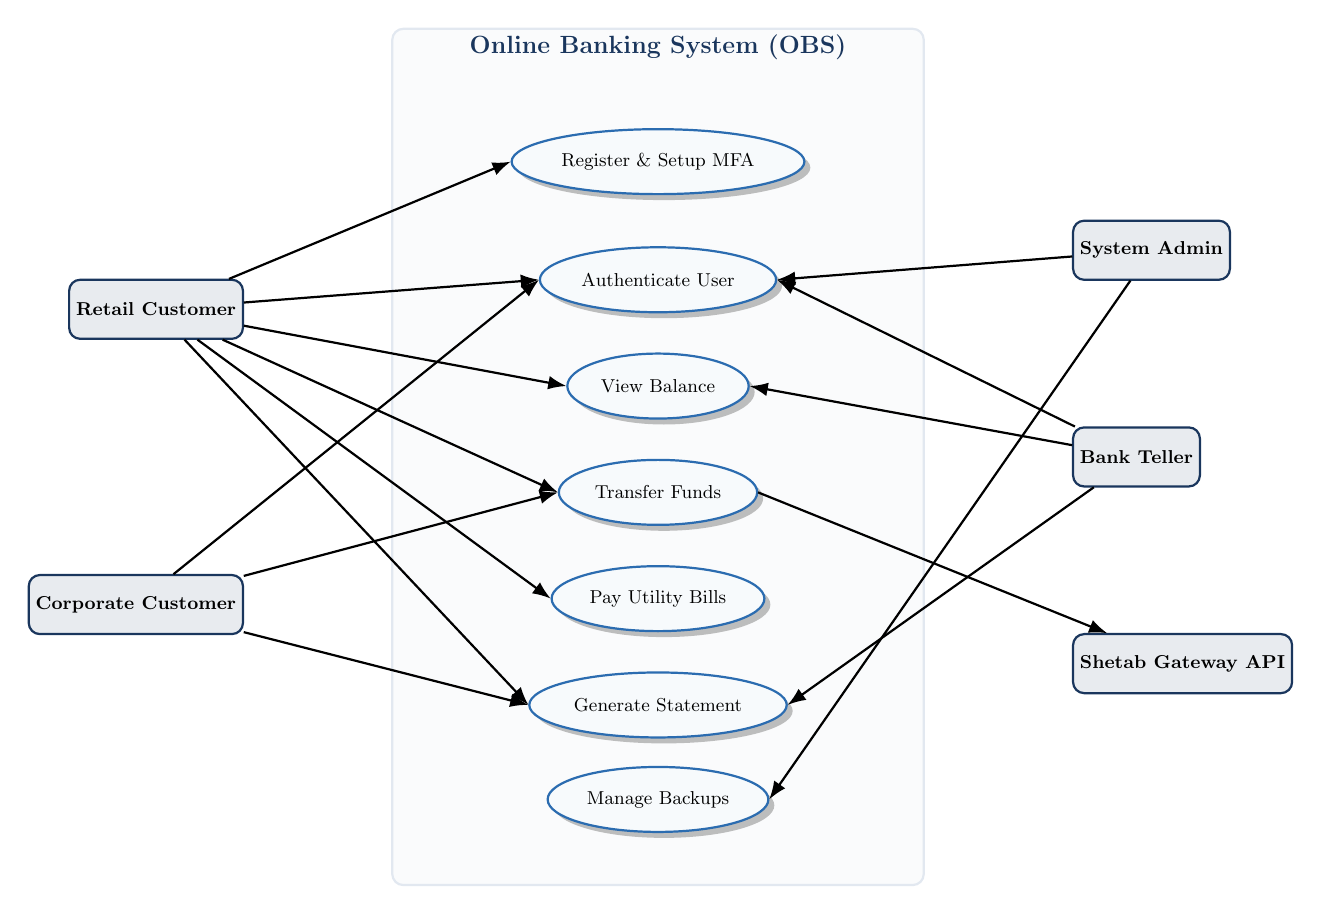
\begin{tikzpicture}[
    scale=0.75, transform shape, % Adjusted scale for perfect fit
    node distance=1.5cm and 2.5cm,
    usecase/.style={ellipse, draw=secondaryblue, fill=lightbg, minimum width=2.8cm, minimum height=1.1cm, align=center, font=\small, thick, drop shadow},
    actor/.style={rectangle, draw=primaryblue, fill=primaryblue!10, minimum width=2cm, minimum height=1cm, rounded corners, font=\bfseries\small, thick},
    boundary/.style={rectangle, draw=bordergray, fill=primaryblue!2, minimum width=9cm, minimum height=14.5cm, thick, rounded corners}
]

    % Draw System Boundary
    \node (sys) [boundary, label={[anchor=north, font=\large\bfseries, text=primaryblue]north:Online Banking System (OBS)}] {};
    
    % Left Actors (Primary)
    \node (cust) [actor, left=of sys.west, yshift=2.5cm] {Retail Customer};
    \node (corp) [actor, left=of sys.west, yshift=-2.5cm] {Corporate Customer};
    
    % Right Actors (Supporting)
    \node (admin) [actor, right=of sys.east, yshift=3.5cm] {System Admin};
    \node (teller) [actor, right=of sys.east, yshift=0cm] {Bank Teller};
    \node (shetab) [actor, right=of sys.east, yshift=-3.5cm] {Shetab Gateway API};

    % Use Cases inside Boundary
    \node (uc_reg) [usecase, parent anchor=center] at (0, 5) {Register \& Setup MFA};
    \node (uc_auth) [usecase] at (0, 3) {Authenticate User};
    \node (uc_bal) [usecase] at (0, 1.2) {View Balance};
    \node (uc_trans) [usecase] at (0, -0.6) {Transfer Funds};
    \node (uc_bill) [usecase] at (0, -2.4) {Pay Utility Bills};
    \node (uc_rep) [usecase] at (0, -4.2) {Generate Statement};
    \node (uc_sys) [usecase] at (0, -5.8) {Manage Backups};

    % Draw Associations - Customer
    \draw [thick, -{Latex}] (cust) -- (uc_reg.west);
    \draw [thick, -{Latex}] (cust) -- (uc_auth.west);
    \draw [thick, -{Latex}] (cust) -- (uc_bal.west);
    \draw [thick, -{Latex}] (cust) -- (uc_trans.west);
    \draw [thick, -{Latex}] (cust) -- (uc_bill.west);
    \draw [thick, -{Latex}] (cust) -- (uc_rep.west);

    % Draw Associations - Corporate
    \draw [thick, -{Latex}] (corp) -- (uc_auth.west);
    \draw [thick, -{Latex}] (corp) -- (uc_trans.west);
    \draw [thick, -{Latex}] (corp) -- (uc_rep.west);

    % Draw Associations - Admin
    \draw [thick, -{Latex}] (admin) -- (uc_auth.east);
    \draw [thick, -{Latex}] (admin) -- (uc_sys.east);

    % Draw Associations - Teller
    \draw [thick, -{Latex}] (teller) -- (uc_auth.east);
    \draw [thick, -{Latex}] (teller) -- (uc_bal.east);
    \draw [thick, -{Latex}] (teller) -- (uc_rep.east);

    % Draw Associations - Shetab
    \draw [thick, -{Latex}] (uc_trans.east) -- (shetab);

\end{tikzpicture}
\caption{UML Use Case Diagram: User boundaries and actors mapping.}
\label{fig:use_case}
\end{figure}

\newpage
\subsection{UML Sequence Diagram (Domestic Fund Transfer Workflow)}
The sequence diagram below represents the step-by-step messaging workflow between system components during a domestic fund transfer transaction.

\begin{figure}[H]
\centering
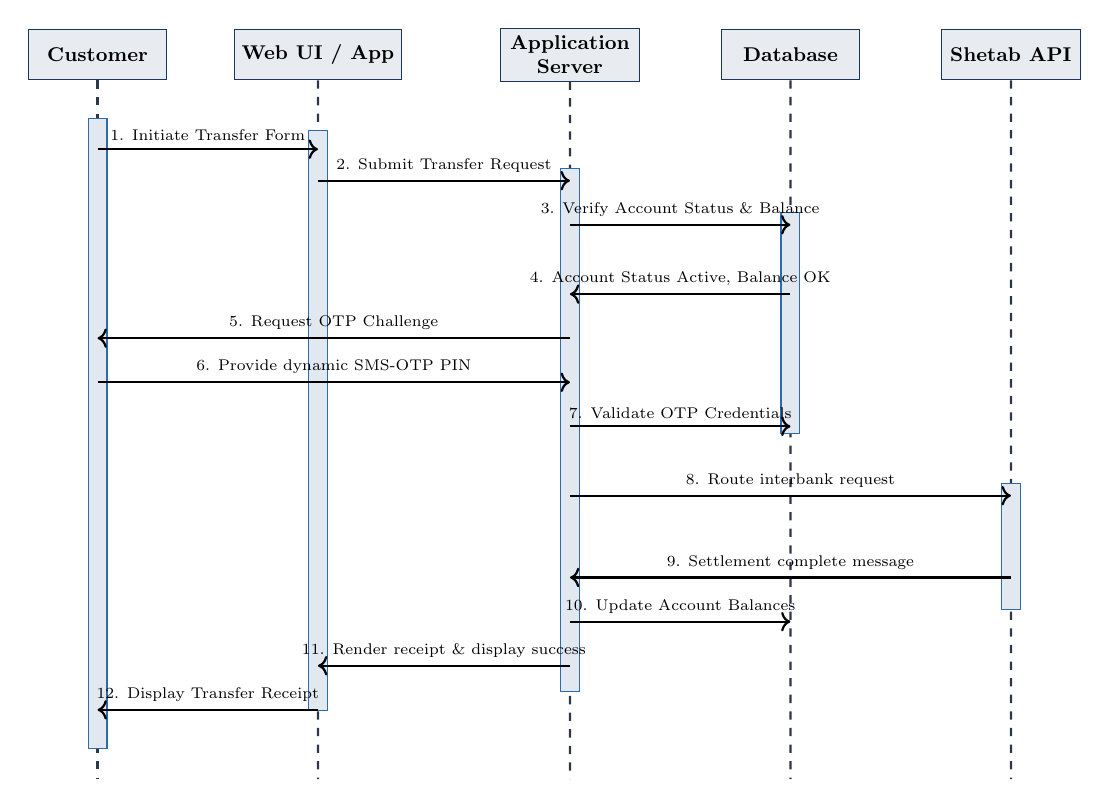
\begin{tikzpicture}[
    scale=0.8, transform shape, % Adjusted scale for perfect fit
    node distance=1.5cm,
    participant/.style={rectangle, draw=primaryblue, fill=primaryblue!10, minimum width=2.2cm, minimum height=0.8cm, font=\bfseries\small, align=center},
    lifeline/.style={dashed, draw=darkgray, thick},
    act/.style={rectangle, draw=secondaryblue, fill=bordergray, minimum width=0.3cm}
]

    % Draw Lifelines / Participants
    \node (cust) [participant] at (0, 0) {Customer};
    \node (ui) [participant] at (3.5, 0) {Web UI / App};
    \node (serv) [participant] at (7.5, 0) {Application\\Server};
    \node (db) [participant] at (11, 0) {Database};
    \node (shetab) [participant] at (14.5, 0) {Shetab API};
    
    % Vertical Lines
    \draw [lifeline] (cust) -- (0, -11.5);
    \draw [lifeline] (ui) -- (3.5, -11.5);
    \draw [lifeline] (serv) -- (7.5, -11.5);
    \draw [lifeline] (db) -- (11, -11.5);
    \draw [lifeline] (shetab) -- (14.5, -11.5);

    % Activation Blocks
    \node (act_cust) [act, minimum height=10cm, anchor=north] at (0, -1) {};
    \node (act_ui) [act, minimum height=9.2cm, anchor=north] at (3.5, -1.2) {};
    \node (act_serv) [act, minimum height=8.3cm, anchor=north] at (7.5, -1.8) {};
    \node (act_db) [act, minimum height=3.5cm, anchor=north] at (11, -2.5) {};
    \node (act_shetab) [act, minimum height=2.0cm, anchor=north] at (14.5, -6.8) {};

    % Sequence Messages
    \draw [->, thick] (0, -1.5) -- node [above, font=\scriptsize] {1. Initiate Transfer Form} (3.5, -1.5);
    \draw [->, thick] (3.5, -2.0) -- node [above, font=\scriptsize] {2. Submit Transfer Request} (7.5, -2.0);
    
    \draw [->, thick] (7.5, -2.7) -- node [above, font=\scriptsize] {3. Verify Account Status \& Balance} (11, -2.7);
    \draw [<-, thick] (7.5, -3.8) -- node [above, font=\scriptsize] {4. Account Status Active, Balance OK} (11, -3.8);
    
    \draw [->, thick] (7.5, -4.5) -- node [above, font=\scriptsize] {5. Request OTP Challenge} (0, -4.5);
    \draw [->, thick] (0, -5.2) -- node [above, font=\scriptsize] {6. Provide dynamic SMS-OTP PIN} (7.5, -5.2);
    
    \draw [->, thick] (7.5, -5.9) -- node [above, font=\scriptsize] {7. Validate OTP Credentials} (11, -5.9);
    
    \draw [->, thick] (7.5, -7.0) -- node [above, font=\scriptsize] {8. Route interbank request} (14.5, -7.0);
    \draw [<-, thick] (7.5, -8.3) -- node [above, font=\scriptsize] {9. Settlement complete message} (14.5, -8.3);
    
    \draw [->, thick] (7.5, -9.0) -- node [above, font=\scriptsize] {10. Update Account Balances} (11, -9.0);
    \draw [->, thick] (7.5, -9.7) -- node [above, font=\scriptsize] {11. Render receipt \& display success} (3.5, -9.7);
    \draw [->, thick] (3.5, -10.4) -- node [above, font=\scriptsize] {12. Display Transfer Receipt} (0, -10.4);

\end{tikzpicture}
\caption{UML Sequence Diagram: Chronological flow of domestic fund transfer transaction.}
\label{fig:sequence}
\end{figure}

\newpage
% =========================================================================
% SECTION 6: REQUIREMENTS TRACEABILITY & VERIFICATION MATRIX
% =========================================================================
\section{Requirements Traceability \& Verification Matrix}
This section contains the Requirements Traceability Matrices (RTM) for the system. Each requirement is mapped to its priority category, the recommended verification method (Test, Demonstration, Inspection, or Analysis), and a specific testing scenario to verify compliance.

\subsection{Functional Requirements Traceability Matrix}
The matrix below maps the functional requirements to their respective verification plans.

\begin{table}[H]
\centering
\caption{Online Banking System - Functional Traceability Matrix}
\label{tab:functional_rtm}
\small
\begin{tabular}{p{2.2cm} p{1.6cm} p{3.2cm} p{2.8cm} p{5.2cm}}
\toprule
\textbf{Req. ID} & \textbf{Priority} & \textbf{Category} & \textbf{Verification Method} & \textbf{Verification / Testing Scenario} \\ \midrule
\textbf{OBS-FR-01} & Must & Authentication & Demonstration & Verify new account signup flows and database hash check. \\ \midrule
\textbf{OBS-FR-02} & Must & Authentication & Test & Verify MFA TOTP/SMS challenge upon credential matching. \\ \midrule
\textbf{OBS-FR-03} & Must & Authorization & Test & Verify RBAC menu rendering and endpoint access rules. \\ \midrule
\textbf{OBS-FR-04} & Should & Authorization & Demonstration & Verify automatic token invalidation after 10 min idle time. \\ \midrule
\textbf{OBS-FR-05} & Must & Data Processing & Test & Run concurrent transaction updates to verify ACID locks. \\ \midrule
\textbf{OBS-FR-06} & Must & Data Processing & Inspection & Static analysis check of form parsing and SQLi/XSS filters. \\ \midrule
\textbf{OBS-FR-07} & Should & UI/UX & Demonstration & Visual rendering checks across various browser viewport widths. \\ \midrule
\textbf{OBS-FR-08} & Should & UI/UX & Inspection & Run screen-reader compliance check (WCAG 2.1 AA checklist). \\ \midrule
\textbf{OBS-FR-09} & Must & Reporting & Test & Initiate statement generation and measure time-to-download. \\ \midrule
\textbf{OBS-FR-10} & Could & Reporting & Demonstration & Check cron trigger at month-end and confirm PDF attachment delivery. \\ \midrule
\textbf{OBS-FR-11} & Must & Third-Party & Test & Verify Shetab API response and cert handshake. \\ \midrule
\textbf{OBS-FR-12} & Must & Third-Party & Demonstration & Confirm asynchronous SMS delivery upon transfers $>$ \$10.00. \\ \midrule
\textbf{OBS-FR-13} & Should & Error Handling & Demonstration & Trigger timeout exception and confirm modal text display. \\ \midrule
\textbf{OBS-FR-14} & Must & Error Handling & Inspection & Inspect log output JSON format and error level fields. \\ \midrule
\textbf{OBS-FR-15} & Must & Backup \& Restore & Inspection & Verify backup snapshot cron job and encryption keys at rest. \\ \midrule
\textbf{OBS-FR-16} & Must & Backup \& Restore & Demonstration & Initiate failover and verify standby site active state transition. \\ \midrule
\textbf{OBS-FR-17} & Could & Authentication & Test & Test SAML/OAuth redirect flows with external provider IDP. \\ \midrule
\textbf{OBS-FR-18} & Could & Data Processing & Test & Query payee database and check return latency under load. \\ \midrule
\textbf{OBS-FR-19} & Should & Third-Party & Test & Trigger balance threshold drop and confirm notification dispatch. \\ \midrule
\textbf{OBS-FR-20} & Should & Error Handling & Demonstration & Submit a support ticket and check operator inbox queue. \\ \bottomrule
\end{tabular}
\end{table}

\newpage

\subsection{Non-Functional Requirements Traceability Matrix}
The matrix below maps the non-functional requirements to their respective verification scenarios and criteria.

\begin{table}[H]
\centering
\caption{Online Banking System - Non-Functional Traceability Matrix}
\label{tab:nonfunctional_rtm}
\small
\begin{tabular}{p{2.2cm} p{1.6cm} p{3.2cm} p{2.8cm} p{5.2cm}}
\toprule
\textbf{Req. ID} & \textbf{Priority} & \textbf{Category} & \textbf{Verification Method} & \textbf{Verification / Testing Scenario} \\ \midrule
\textbf{OBS-NFR-01} & Should & Usability & Test & Usability studies (measure signup setup duration/onboarding time). \\ \midrule
\textbf{OBS-NFR-02} & Must & Security & Inspection & Audit system volumes and API ports to confirm AES-256/TLS 1.3. \\ \midrule
\textbf{OBS-NFR-03} & Must & Security & Inspection & Verify database hash salt strength and Argon2id config parameters. \\ \midrule
\textbf{OBS-NFR-04} & Must & Reliability & Test & Induce process kills mid-transfer and verify rollback completion. \\ \midrule
\textbf{OBS-NFR-05} & Must & Performance & Test & Load test home page and measure response times under SLA limits. \\ \midrule
\textbf{OBS-NFR-06} & Should & Scalability & Test & JMeter/Gatling simulation scaling up to 100,000 active sessions. \\ \midrule
\textbf{OBS-NFR-07} & Must & Availability & Analysis & Review monthly SLA reports and check scheduled downtime logs. \\ \midrule
\textbf{OBS-NFR-08} & Should & Compatibility & Demonstration & Run automated Selenium grid cross-browser compatibility tests. \\ \midrule
\textbf{OBS-NFR-09} & Must & Reliability & Test & Run bi-weekly database backup restore automation verification checks. \\ \midrule
\textbf{OBS-NFR-10} & Should & Usability & Test & Measure timestamp lag from ticket submission to operator routing. \\ \midrule
\textbf{OBS-NFR-11} & Must & Security \& Compliance & Inspection & Verify PCI-DSS audit parameters and 7-year storage key rotations. \\ \midrule
\textbf{OBS-NFR-12} & Should & Maintainability & Analysis & Check SonarQube dashboards to confirm code test coverage $\ge$ 85\%. \\ \bottomrule
\end{tabular}
\end{table}

\end{document}
